% Example drawings to help explain the VSEPR atom model to high school
% students. Although the actual model is three dimensional, these drawings
% are deliberately presented as two dimensional to gently introduce them to the
% concepts, before advancing to three dimensional models.
%
% Authors: Berteun Damman & Arne Rhrs

\documentclass{article}
\usepackage{verbatim}

\begin{comment}
:Title: Atoms and orbitals


Example drawings to help explain the `VSEPR atom model`_ to high school
students. Although the actual model is three dimensional, these drawings
are deliberately presented as two dimensional to gently introduce them to the
concepts, before advancing to three dimensional models.

.. _VSEPR atom model: http://en.wikipedia.org/wiki/VSEPR_theory

\end{comment}
\usepackage{tikz}
%%%% BRM HACKED SOURCE
%%%%\usepackage[version=3]{mhchem}
\def\ce#1{#1}


\pgfdeclarelayer{background}
\pgfdeclarelayer{foreground}
\pgfsetlayers{background,main,foreground}

% For black & white suggestions are black!95 for the electron
% and a white background, or a simple shade for the orbitals.
\colorlet{electron}{blue!75}
\tikzset{orbital/.style={thick,draw=blue,fill opacity=.60}}
% Styles for orbitals with 0, 1 and 2 atoms respectively.
\tikzset{orbital 0/.style={orbital,fill=blue!25}}
\tikzset{orbital 1/.style={orbital,fill=blue!66}}
\tikzset{orbital 2/.style={orbital,fill=blue}}
\tikzset{atomcore/.style={shape=circle,thick,draw=red!40,minimum size=7mm,
    font=\large\color{red!70!gray},fill=red!20,inner sep=0pt}}

\def\orbheight{1.2}
\def\orbwidth{.6}

% Parameters: #1 Rotation of the orbital
%             #2 Coordinate where the orbital should be attached
%             #3 Number of electrons to draw in the orbital
\newcommand{\orbital}[3]{
    \begin{scope}[rotate=#1,shift=(#2)]
        % These points define the curve for the orbital.
        \coordinate (c1) at (-\orbwidth, .6 * \orbheight);
        \coordinate (c2) at (-\orbwidth, \orbheight);
        \coordinate (c3) at (\orbwidth, \orbheight);
        \coordinate (c4) at (\orbwidth, .6 * \orbheight);
        \coordinate (top) at (0,\orbheight);

        %Coordinates of the electrons
        \coordinate (e1) at (0, 0.45*\orbheight);
        \coordinate (e2) at (0, 0.75*\orbheight);
    \end{scope}

  % These are drawn on a background layer, so orbitals
  % can overlap without covering the electrons, which
  % visualises the role electrons play in chemical bonds.
  \begin{pgfonlayer}{background}
      \draw[orbital #3] (#2) .. controls (c1) and (c2) .. (top) ..
            controls (c3) and (c4) .. (#2);
  \end{pgfonlayer}

  % Draw the electrons
  \ifnum#3>0
      \foreach \n in {1,...,#3} {
          \shade[ball color=electron] (e\n) circle (1mm);
      }
  \fi
}

% This allows to quickly place an atom.
% Parameters: #1 (Optional) Name of the center node
%             #2 Text for the center node
%             #3 A list of rotation-angle/anchor/number of electrons
\newcommand{\Atom}[3][AtomNode]{
  \node[atomcore] (#1) {\ce{#2}};
  \foreach \ang/\anchor/\n in {#3} {
      \orbital{\ang}{#1.\anchor}{\n}
  }
}

\begin{document}
    \pagestyle{empty}
    
    
% Note: Cells of matrices cannot contain layered pictures,
% therefore we use some old-fashioned scopes.
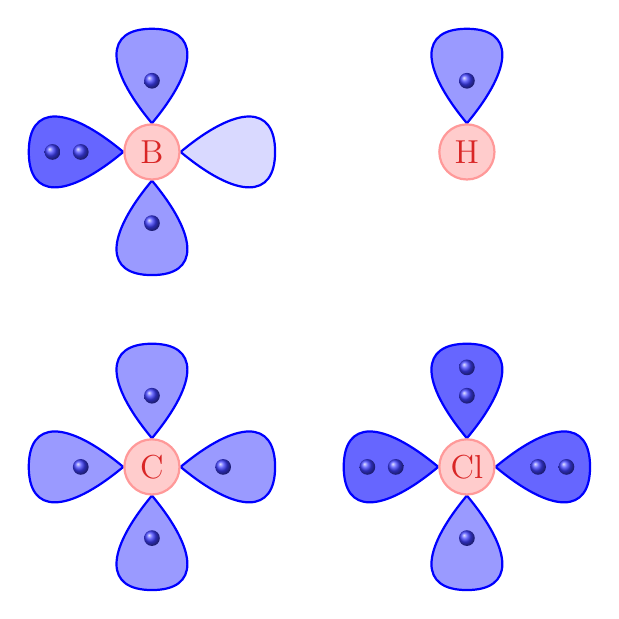
\begin{tikzpicture}
    \Atom{B}{90/west/2,0/north/1,270/east/0,180/south/1}
    \begin{scope}[xshift=4cm]
        \Atom{H}{0/north/1}
    \end{scope}
    \begin{scope}[yshift=-4cm]
        \Atom{C}{90/west/1,0/north/1,270/east/1,180/south/1}
        \begin{scope}[xshift=4cm]
            \Atom{Cl}{90/west/2,0/north/2,270/east/2,180/south/1}
        \end{scope}
    \end{scope}
\end{tikzpicture}
\medskip

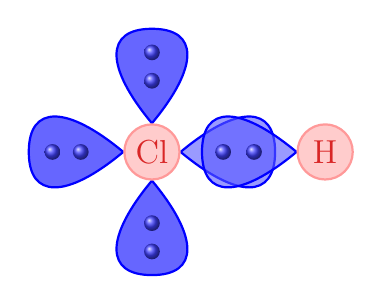
\begin{tikzpicture}
    \Atom{Cl}{90/west/2,0/north/2,270/east/1,180/south/2}
    \begin{scope}[xshift=2.2cm]
        \Atom{H}{90/west/1}
    \end{scope}
\end{tikzpicture}

%% BRM Hack; there's some kind of picture duplication going on...
%\end{document}
\medskip

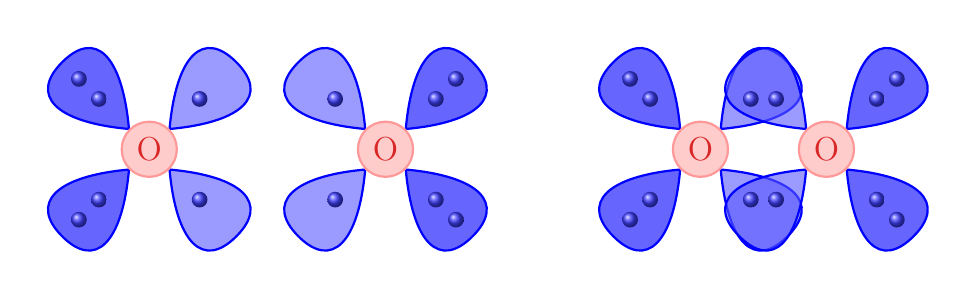
\begin{tikzpicture}
    \Atom{O}{45/north west/2,315/north east/1,225/south east/1,135/south west/2}
    \begin{scope}[xshift=3.0cm]
        \Atom{O}{45/north west/1,315/north east/2,225/south east/2,135/south west/1}
    \end{scope}

    \begin{scope}[xshift=7.0cm]
        \Atom{O}{45/north west/2,315/north east/1,225/south east/1,135/south west/2}
        \begin{scope}[xshift=1.6cm]
            \Atom{O}{45/north west/1,315/north east/2,225/south east/2,135/south west/1}
        \end{scope}
    \end{scope}
\end{tikzpicture}

\end{document}
